\documentclass[sigplan,screen]{acmart}
\setcopyright{rightsretained}
\acmPrice{}
\acmDOI{}
\acmYear{2023}
\copyrightyear{2023}
\acmConference{PEPM}{2023}{Boston}

\bibliographystyle{ACM-Reference-Format}
\citestyle{acmauthoryear}   %% For author/year citations

% 12 pages

\usepackage[english]{babel}
\usepackage{amsthm}
\usepackage{graphicx,color}
\usepackage{subcaption}
\usepackage{braket}
\usepackage{minted}
\usepackage{yquant}
\usepackage{multirow}
\usepackage{enumitem}
\usepackage{tikz}
\usetikzlibrary{quantikz,fit,quotes,svg.path}

\newcommand{\h}[1]{\mintinline{haskell}{#1}}

\newcommand{\x}{\textsc{x}}
\newcommand{\cx}{\textsc{cx}}
\newcommand{\ccx}{\textsc{ccx}}
\newcommand{\cccx}{\textsc{cccx}}
\newcommand{\qket}[1]{\ket{\tilde{#1}}}
\newcommand{\preim}[2]{\{\cdot\stackrel{#1}{\longleftarrow}{#2}\}}
\newcommand{\finset}[1]{[\mathbf{#1}]}
\newcommand{\red}[1]{{\color{red}{#1}}}
\newcommand{\todo}[1]{\fbox{\begin{minipage}{40em}{\red{#1}}\end{minipage}}}

\newcommand{\Cplx}{\ensuremath{\mathbb{C}}}
\newcommand{\Bool}{\ensuremath{\mathbb{B}}}

\theoremstyle{definition}
\newtheorem*{insight}{Insight}
\newtheorem*{signif}{Significance}

%%%%%%%%%%%%%%%%%%%%%%%%%%%%%%%%%%%%%%%%%%%%%%%%%%%%%%%%%%%%%%%%%%%%%%%%%
\begin{document}

\title[Symbolic Quantum Execution]{Symbolic Execution of \\
  Hadamard-Toffoli Quantum Circuits}

\author{Jacques Carette}
\orcid{0000-0001-8993-9804}
\affiliation{
  \department{Department of Computing and Software}
  \institution{McMaster University}
  \city{Hamilton}
  \postcode{L8S 4K1}
  \country{Canada}
}
\email{carette@mcmaster.ca}

\author{Gerardo Ortiz}
\orcid{0000-0003-3254-4494}
\affiliation{
  \department{Department of Physics}
  \institution{Indiana University}
  \city{Bloomington}
  \postcode{47408}
  \country{USA}
}
\email{ortizg@iu.edu}

\author{Amr Sabry}
\orcid{0000-0002-1025-7331}
\affiliation{
  \department{Department of Computer Science}
  \institution{Indiana University}
  \city{Bloomington}
  \postcode{47408}
  \country{USA}
}
\email{sabry@indiana.edu}

\begin{abstract}
  The simulation of quantum programs by classical computers is a critical endeavor
  for several reasons: it provides proof-of-concept validation of
  quantum algorithms; it provides opportunities to experiment with new
  programming abstractions suitable for the quantum domain, and most
  significantly it is a way to explore the elusive boundary at which a
  quantum advantage may materialize. Here, we show that traditional
  techniques of symbolic evaluation and partial evaluation yield
  surprisingly efficient classical simulations for some instances of
  textbook quantum algorithms that include the Deutsch, Deutsch-Jozsa,
  Bernstein-Vazirani, Simon, Grover, and Shor's algorithms. The success
  of traditional partial evaluation techniques in this domain is due
  to one simple insight: the quantum bits used in these algorithms can
  be modeled by a symbolic boolean variable while still keeping track
  of the correlations due to superposition and entanglement. More
  precisely, the system of constraints generated over the symbolic
  variables contains all the necessary quantum correlations and hence
  the answer to the quantum algorithms. With a few programming tricks
  explained in the paper, quantum circuits with millions of gates can
  be symbolically executed in seconds. Paradoxically, other circuits
  with as few as a dozen gates take exponential time. We reflect on
  the significance of these results in the conclusion.
\end{abstract}

\begin{CCSXML}
<ccs2012>
   <concept>
       <concept_id>10003752.10010124</concept_id>
       <concept_desc>Theory of computation~Semantics and reasoning</concept_desc>
       <concept_significance>500</concept_significance>
       </concept>
   <concept>
       <concept_id>10003752.10010124.10010131.10010134</concept_id>
       <concept_desc>Theory of computation~Operational semantics</concept_desc>
       <concept_significance>500</concept_significance>
       </concept>
   <concept>
       <concept_id>10010147.10010148.10010149</concept_id>
       <concept_desc>Computing methodologies~Symbolic and algebraic algorithms</concept_desc>
       <concept_significance>500</concept_significance>
       </concept>
   <concept>
       <concept_id>10010405.10010432.10010441</concept_id>
       <concept_desc>Applied computing~Physics</concept_desc>
       <concept_significance>500</concept_significance>
       </concept>
 </ccs2012>
\end{CCSXML}

\ccsdesc[500]{Theory of computation~Semantics and reasoning}
\ccsdesc[500]{Theory of computation~Operational semantics}
\ccsdesc[500]{Computing methodologies~Symbolic and algebraic algorithms}
\ccsdesc[500]{Applied computing~Physics}


\keywords{{quantum computation}, {partial evaluation}, {symbolic
    evaluation}, {retrodictive quantum computing}, {algebraic normal
    form}, {boolean circuits}, {quantum oracles}}
\maketitle

%%%%%%%%%%%%%%%%%%%%%%%%%%%%%%%%%%%%%%%%%%%%%%%%%%%%%%%%%%%%%%%%%%%%%%%%%
\section{Introduction}

Classical models of computation are widely believed to be
less powerful than quantum ones. Nevertheless, it is of utmost
importance to establish when, for a given problem,  a classical
algorithm is as resource efficient as its quantum counterpart.
In this paper we address this question from a new angle, apparently,
not explored before. We consider traditional techniques of
symbolic and partial evaluation to classically simulate quantum
circuits assembled from Hadamard and Toffoli gates. The latter
constitutes a set of quantum gates that is known to be
computationally universal~\cite{aharonov:toffolihadamard}.

Using partial evaluation to optimize reversible or quantum circuits is
not itself a novel idea (see, e.g.,
\cite{10.1007/978-3-319-63390-9_1,10.1145/1929501.1929506}). What
distinguishes our approach are the following two important
observations. Firstly, since quantum algorithms are reversible,
depending on the problem at hand, one can always take advantage of
``backwards-in-time'' execution (known as \emph{retrodictive}
execution~\cite{RevModPhys.27.179,sym13040586,retrodictive,Aharonov2008}). Secondly,
since Hadamard is a purely quantum gate, with no classical
counterpart, we need to eliminate the superposition generated by such
a gate and replace it with a symbolic variable that preserves the
relevant quantum correlations. This turns out to be straightforward
for instances of Hadamard gates used in the first stage of quantum
algorithms to introduce a uniform superposition of all relevant
inputs. These two new ideas, while not expressive enough to model arbitrary
quantum computations, are effective for instances of standard examples
of quantum algorithms.

Our approach can be broadly related to other
classical approaches to reason about subsets of quantum circuits,
e.g., without entanglement~\cite{10.1145/3563309}, or for Clifford
groups~\cite{osti_319738,DBLP:journals/corr/abs-1805-06908}, but with
different tradeoffs: we allow arbitrary entanglement at the cost of
sometimes generating exponentially large equations and we deal
with an incomparable set of gates compared to the Clifford group. 

\paragraph*{Outline.} We begin in Sec.~\ref{sec2} with background
information on quantum computing with a focus on the idea of
representing a class of qubit states using symbolic
variables. Sec.~\ref{anf} shows how standard quantum gates can be
modeled using this symbolic representation by using the algebraic
normal form (ANF) of boolean formulae. Sec.~\ref{sec3} reviews the
family of quantum algorithms that is the focus of our approach and
highlights the new perspective brought by symbolic execution. Our main
technical contribution, the design and implementation, of a symbolic
evaluator for Hadamard-Toffoli quantum circuits, is explained in
Sec.~\ref{sec4}. The next section (Sec.~\ref{sec5}) includes a
complexity analysis and a performance evaluation of our symbolic
evaluator on major textbook algorithms. Sec.~\ref{sec6} concludes with
a summary and a discussion of the broader implications of our approach
to the understanding of the classical / quantum performance
characteristics. Our code is available online\footnote{
  \url{https://github.com/JacquesCarette/Retrodictive/tree/main/execution/RetroPE}}.

%%%%%%%%%%%%%%%%%%%%%%%%%%%%%%%%%%%%%%%%%%%%%%%%%%%%%%%%%%%%%%%%%%%%%%%%%
\section{Qubits as Symbolic Variables}
\label{sec2}

The general state of a quantum bit (qubit) is mathematically modeled
using an equation parameterized by two angles $\theta$ and $\phi$ as
follows:
\[
\cos{\frac{\theta}{2}} \ket{0} + e^{i\phi} \sin{\frac{\theta}{2}} \ket{1} .
\]
The description models the fact that the qubit is in a superposition
of false $\ket{0}$ and true $\ket{1}$. The angle $\theta$
determines the relative amplitudes of false and true and the angle
$\phi$ determines the relative phase between them. A particular case
when $\theta = \pi/2$ and $\phi=0$ is ubiquitous in quantum
algorithms. In those cases, the general representation reduces to:
\[
1/\sqrt{2}~ (\ket{0} + \ket{1} ) ,
\]
which represents a qubit in an equal superposition of false and
true and with no relative phase between them.

The reason this particular case is distinguished is because a rather
common template for quantum algorithms is to start with qubits
initialized to $\ket{0}$ and immediately apply a Hadamard $H$ transformation
whose action is:
\[
  \ket{0} \mapsto 1/\sqrt{2} ~(\ket{0} + \ket{1}) .
\]
This superposition is then further manipulated depending on the
algorithm in question.

\begin{figure}[t]
\begin{center}
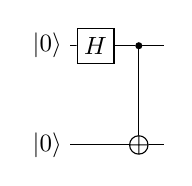
\begin{tikzpicture}[scale=0.9]
   \begin{yquant*}[register/minimum height=1.3cm]
   qubit {$\ket0$} x;
   qubit {$\ket0$} y;
   box {$H$} x;
   cnot y | x;
  \end{yquant*}
\end{tikzpicture}
\qquad\qquad
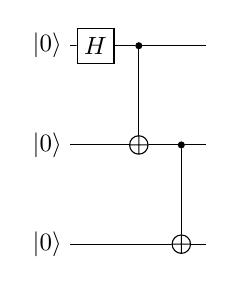
\begin{tikzpicture}[scale=0.9]
 \begin{yquant*}[register/minimum height=1.3cm]
   qubit {$\ket0$} x;
   qubit {$\ket0$} y;
   qubit {$\ket0$} z;
   box {$H$} x;
   cnot y | x;
   cnot z | y;
  \end{yquant*}
\end{tikzpicture}
\end{center}
\caption{\label{fig:bell2}Bell and GHZ States}
\end{figure}

\begin{figure*}[t]
  \centering
\begin{subfigure}[b]{.25\textwidth}
    \centering
    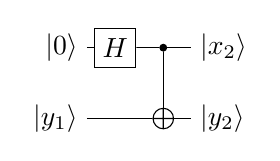
\begin{tikzpicture}[scale=1.0]
   \begin{yquant*}[register/minimum height=0.8cm]
   qubit {$\ket{0}$} x;
   qubit {$\ket{y_1}$} y;
   box {$H$} x;
   cnot y | x;
   output {$\ket{x_2}$} x;
   output {$\ket{y_2}$} y;
  \end{yquant*}
\end{tikzpicture}
\caption{\label{fig:bellqcore}Bell circuit}
\end{subfigure}
\qquad\qquad
\begin{subfigure}[b]{.25\textwidth}
    \centering
    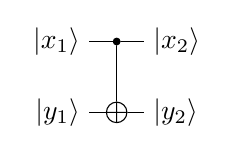
\begin{tikzpicture}[scale=1.0]
   \begin{yquant*}[register/minimum height=0.8cm]
   qubit {$\ket{x_1}$} x;
   qubit {$\ket{y_1}$} y;
   cnot y | x;
   output {$\ket{x_2}$} x;
   output {$\ket{y_2}$} y;
  \end{yquant*}
\end{tikzpicture}
\caption{\label{fig:bellccore}Symbolic variant}
\end{subfigure}
\caption{\label{fig:bellall}A conventional quantum circuit for
  generating a Bell state (a); its classical symbolic variant (b).}
\end{figure*}

Our observation is that a qubit in the special superposition
$1/\sqrt{2} ~(\ket{0} + \ket{1} )$ is, computationally speaking,
indistinguishable from a symbolic boolean variable with an unknown
value in the same sense used in symbolic evaluation of classical
programs~\cite{10.1145/390016.808445,10.1145/360248.360252,howden,10.1145/800191.805647,10.1145/3182657}.
First, the superposition is not observable. The only way to
observe the qubit is via a measurement which collapses the state to be
either false or true with equal probability. Second, and more
significantly, this remarkably simple observation is quite robust even
in the presence of multiple, possibly entangled, qubits.

To see this, consider the conventional quantum circuits for creating
the maximally entangled Bell and GHZ states in
Fig.~\ref{fig:bell2}. On the left, the circuit generates the Bell
state $(1/\sqrt{2})~ (\ket{00} + \ket{11})$ as follows. First the state
evolves from $\ket{00}$ to $(1/\sqrt{2})~ (\ket{00} + \ket{10})$. Then
we apply the \cx-gate whose action is to negate the second qubit when
the first one is true. By using the symbol $x$ for $H\ket{0}$, the
input to the \cx-gate is $\ket{x0}$. A simple case analysis shows that
the action of \cx-gate on inputs $\ket{xy}$ is $\ket{x(x \oplus y)}$
where $\oplus$ is the exclusive-or boolean operation. In other words,
the \cx-gate transforms $\ket{x0}$ to $\ket{xx}$. Since any
measurement of the Bell state must produce either 00 or 11,
a symbolic state that shares the same name in two positions
accurately represents the entangled Bell state. Similarly,
for the GHZ circuit on the right of Fig.~\ref{fig:bell2}, the state
after the Hadamard gate is $\ket{x00}$ which evolves to $\ket{xx0}$
and then to $\ket{xxx}$ again accurately capturing the entanglement
correlations.

Because quantum circuits are reversible, i.e., executable forwards
and backwards, the introduction of symbolic variables opens a host of
new exciting possibilities beyond conventional (classical) symbolic
evaluation: for a given quantum circuit \emph{any mixture of inputs and outputs
can be deemed symbolic}. For example, consider again the Bell circuit in
Fig.~\ref{fig:bellall} but with an arbitrary initial value for the second
qubit. The right subfigure (Fig.~\ref{fig:bellccore}) removes the
explicit use of $H\ket{0}$ and replaces the top qubit with another
symbolic variable. Because quantum circuits are reversible, we can, at
this point, ``partially evaluate'' the circuit under various
regimes. For example, we can set $y_1=0$ and $y_2=1$ and ask about
values of $x_1$ and $x_2$ that would be consistent with this
setting. We can calculate backwards from $\ket{x_21}$ as follows. The
state evolves to $\ket{x_2(1 \oplus x_2)}$ which can be reconciled
with the initial conditions yielding the constraints $x_1=x_2$ and
$1 \oplus x_2 = 0$ whose solutions are $x_1 = x_2 = 1$.

Technically, the problem of symbolic evaluation of our quantum
circuits then reduces to a mixture of partial evaluation, slicing, and
symbolic evaluation. Like with partial evaluation, we have some inputs
dynamic, some static, and a static program. Similarly for slicing, but
with outputs. Our situation is significantly simpler than in both
cases. First, our language is reversible, which makes backwards
evaluation deterministic, unlike for most languages. Second, the
values at each step of circuit execution are boolean functions
manipulated with conditional exclusive-or operations with a
well-understood normal form, ANF, explained next.

%%%%%%%%%%%%%%%%%%%%%%%%%%%%%%%%%%%%%%%%%%%%%%%%%%%%%%%%%%%%%%%%%%%%%%%%%
\section{Algebraic Normal Form (ANF)}
\label{anf}

The circuits we are interested in can all be expressed in terms of
\emph{generalized Toffoli gates} with $n$ control qubits:
$a_0,\cdots,a_{n-1}$ and one target qubit $c$, where the effect is to
leave all the control qubits unchanged and send $c$ to
$c \oplus \bigwedge_i a_i$, the exclusive-or of the target $c$ with
the conjunction of all the control qubits. In fact, we generalize this
further, so that we can control either on a qubit or its negation, by
using pairs of a control qubit and a boolean. In other words, our
gates are specified by a collection $(a_0,b_0),\cdots,(a_{n-1},b_{n-1})$
together with one target qubit $c$; their action is to send the target
qubit to $c \oplus \bigwedge_i \left(a_i == b_i\right)$, the
exclusive-or of the target $c$ with the conjunction of the result of
testing each qubit against its corresponding target boolean. Note that
$\left(a_i == 1\right)$ can be expressed as just $a_i$, and
$\left(a_i == 0\right)$ can be expressed as $1 \oplus a_i$.  Such
generalized Toffoli gates with~$n$ control qubits are called $c^nx$
gates. It is worth noting the following special cases:
\begin{itemize}
  \item for $n=0$, we get the \emph{not} gate \x,
  \item for $n=1$, we get the \emph{controlled not} gate \cx, and
  \item for $n=2$, we get the \emph{controlled controlled not} or the
    conventional \emph{Toffoli} gate \ccx.
\end{itemize}

The \emph{algebraic normal form}~\cite{TOKAREVA20151,10.5555/35517}
(ANF also called ring sum normal form, Zhegalkin normal form or
Reed-Muller expansion) of boolean functions $\Bool^n\rightarrow\Bool$
is the exclusive-or of $\wedge$-clauses where each clause is the
conjunction of 0 or more inputs $x_i$. Note that the conjunction of
$0$ inputs is $1$ and that $1 \oplus F$ is the negation of $F$ which
means that negation is not needed as a separate primitive. It is then
easy to see that generalized Toffoli gates are essentially in ANF and
that symbolic circuit evaluation can proceed by maintaining the ANF
representation of the circuit. Furthermore, circuits that only use \x\
and \cx-gates never generate any conjunctions and hence lead to
formulae that are efficiently solvable
classically~\cite{10.5555/35517,TOKAREVA20151}.

\begin{figure*}[t]
  \centering
\begin{subfigure}[c]{.25\textwidth}
    \centering
    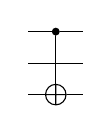
\begin{tikzpicture}[scale=1.0]
   \begin{yquant*}[register/minimum height=0.3cm]
   qubit {} x;
   qubit {} y;
   qubit {} z;
   cnot z | x;
  \end{yquant*}
\end{tikzpicture}
\end{subfigure}
\qquad$\equiv$\qquad
\begin{subfigure}[c]{.25\textwidth}
    \centering
    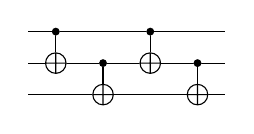
\begin{tikzpicture}[scale=1.0]
   \begin{yquant*}[register/minimum height=0.3cm]
   qubit {} x;
   qubit {} y;
   qubit {} z;
   cnot y | x;
   cnot z | y;
   cnot y | x;
   cnot z | y;
  \end{yquant*}
\end{tikzpicture}
 \end{subfigure}
\caption{\label{fig:cnotopt}A gate equivalence}
\end{figure*}

\begin{figure*}[t]
  \centering
\begin{subfigure}[c]{.25\textwidth}
    \centering
    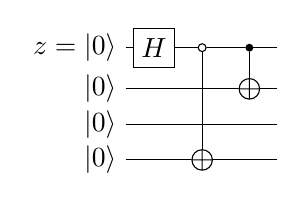
\begin{tikzpicture}[scale=1.0]
   \begin{yquant*}[register/minimum height=0.3cm]
   qubit {$z=\ket{0}$} z;
   qubit {$\ket{0}$} a;
   qubit {$\ket{0}$} b;
   qubit {$\ket{0}$} c;
   box {$H$} z;
   cnot c | ~z;
   cnot a | z;
  \end{yquant*}
\end{tikzpicture}
\end{subfigure}
\qquad$\equiv$\qquad
\begin{subfigure}[c]{.25\textwidth}
    \centering
    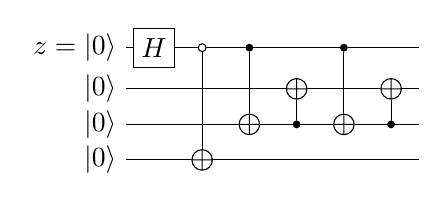
\begin{tikzpicture}[scale=1.0]
   \begin{yquant*}[register/minimum height=0.3cm]
   qubit {$z=\ket{0}$} z;
   qubit {$\ket{0}$} a;
   qubit {$\ket{0}$} b;
   qubit {$\ket{0}$} c;
   box {$H$} z;
   cnot c | ~z;
   cnot b | z;
   cnot a | b;
   cnot b | z;
   cnot a | b;
  \end{yquant*}
\end{tikzpicture}
 \end{subfigure}
\caption{\label{fig:circopt}A circuit equivalence using the gate
  equivalence in Fig.~\ref{fig:cnotopt}}
\end{figure*}

The ANF of a boolean function is unique. This means that two different
circuits implementing the same function have the same symbolic ANF
representation. As a small example, Fig.~\ref{fig:cnotopt} shows an
equivalence that is often useful when only nearest-qubit interactions
are available. Fig.~\ref{fig:circopt} shows two fragments of a circuit
used in Shor's algorithm that each use one side of the equivalence. We
demonstrate, manually, how the ANF symbolic representation of the two
circuits is unique, which explains why a non-optimized circuit with
millions of gates can be efficiently processed if the underlying
function has an efficient circuit representation.

Let's start symbolically evaluating the circuit on the left of
Fig.~\ref{fig:circopt}. Replacing $H\ket{0}$ by $z$ for the top wire, the
initial state for the symbolic execution is $\ket{z000}$.  The white
dot in the graphical representation of the first gate indicates that
the control is active when it is 0. The state proceeds to
$\ket{z00(1\oplus z)}$. The second gate then produces
$\ket{zz0(1\oplus z)}$ as the final state. For the circuit on the
right, symbolic evaluation proceeds as follows:
\[\begin{array}{rcl}
    \ket{z000}  &\mapsto& \ket{z00(1\oplus z)} \\
                &\mapsto& \ket{z0z(1\oplus z)} \\
                &\mapsto& \ket{zzz(1\oplus z)} \\
                &\mapsto& \ket{zz0(1\oplus z)} \\
                &\mapsto& \ket{zz0(1\oplus z)} ,
\end{array}\]
which is the same ANF representation as the first circuit.

To summarize, we never need to residualize a circuit, we can always
get a ``closed form,'' in ANF, for evaluation, whether forward or
backward. Evaluating a circuit in one fixed direction is then quite
standard. A novel approach, enabled by the reversibility of quantum
mechanics, is what we call the \emph{retrodictive} mode of running
circuits, as explained in our preprint \cite{retrodictive} which
further details the quantum and physics side of this work (but
does not speak of the implementation beyond saying that it exists).
In that mode, illustrated in
Fig.~\ref{fig:retroflow} , we start execution in the forward direction
with a fully static collection of inputs in order to partially
determine a possible future; we then execute backwards from the
partially specified possible future (with the unknown values
represented symbolically). This combination of static and dynamic
knowledge of the output produces as its result a \emph{system of
constraints} equating the resulting logical polynomials to the
circuit's inputs. If the system of constraints has a solution, then
that output was feasible. What we will actually see is that for many
quantum circuits, we can ``read off'' the information we need from the
system of constraint themselves, \emph{without needing to actually
solve them}.

%%%%%%%%%%%%%%%%%%%%%%%%%%%%%%%%%%%%%%%%%%%%%%%%%%%%%%%%%%%%%%%%%%%%%%%%%
\section{Quantum Algorithms}
\label{sec3}

Let $\finset{n}$ denote the finite set $\{ 0,1,\ldots,(n-1)\}$. The
parameter~$n$ determines the problem size for all the problems below
(except Deutsch which is a fixed sized problem). In the review below,
we adapt the usual presentation of the
algorithms~\cite{doi:10.1137/S0097539796300921,deutsch,deutschJozsa,365701,doi:10.1137/S0097539795293172,nielsen_chuang_2010,10.1145/237814.237866}
to one better suited to our context. In particular, we focus on the
heart of the algorithm, the quantum oracle, which encapsulates the
underlying boolean function of interest. Furthermore, instead of using
the forward flow of execution using exact quantum superpositions, we
express the problem as one asking for particular properties of the
pre-image of the classical function embedded in the quantum oracle.

\paragraph*{Deutsch.}
The conventional statement of the problem is to determine if a
function $\finset{2} \rightarrow \finset{2}$ is constant or
balanced. In this small case, there are just four possible functions;
the function is balanced if it is the identity or boolean negation,
and is constant otherwise. Equivalently, we can ask about the
pre-image of an arbitrary boolean value (say false), i.e., the set of
inputs that are mapped to false by the function, and check whether the
pre-image has an even or odd number of elements. If the cardinality of
the pre-image is even, i.e., 0 or 2, the function must be constant and
if it is odd, i.e., it contains just one element, the function must be
balanced. 

\paragraph*{Deutsch-Jozsa.}
The problem is a generalization of the previous one: the question is
to determine if a function $\finset{2^{\it n}} \rightarrow \finset{2}$ for
some $n$ is constant or balanced. When expressed as a pre-image
computation, the problem reduces to a query distinguishing the
following three situations about the pre-image of a value in the range
of the function: is the cardinality of the pre-image equal to 0,
$2^n$, or $2^{n-1}$? In the first two cases, the function is constant
and in the last case, the pre-image contains half the values in the
domain indicating that the function is balanced. 

\paragraph*{Bernstein-Vazirani.}
We are given a function $f : \finset{2^{\it n}} \rightarrow \finset{2}$
that hides a secret number $s \in \finset{2^{\it n}}$. We are promised the
function is defined using the binary representations $\sum_i^{n-1}
x_i$ and $\sum_i^{n-1} s_i$ of $x$ and $s$ respectively as follows:
\[
f(x) = \sum_{i=0}^{n-1} s_ix_i \mod{2} \ .
\]
The goal is to determine the secret number $s$.

Expressing the problem as a pre-image calculation is slightly more
involved than in the previous two cases. To determine~$s$, we compute
the pre-image of a value in the range of the function, and then make
$n$ queries to this pre-image. Query $i$ asks whether $2^i$ is a
member of the pre-image and the answer determines bit $i$ of the
secret $s$. Indeed, by definition, $f(2^i) = s_i$ and hence $s_i$ is 1
iff $2^i$ is a member of the pre-image of 1.

\paragraph*{Simon.}
We are given a 2-1 function $f : \finset{2^{\it n}} \rightarrow
\finset{2^{\it n}}$ with the property that there exists an $a$ such $f(x) =
f(x \oplus a)$ for all~$x$; the goal is to determine $a$. When
expressed as a computation of pre-images, the problem statement
becomes the following. Pick an arbitrary $x$ and compute the pre-image
of $f(x)$. It must contain exactly two values one of which is~$x$. The
problem then reduces to finding the other value in the pre-image.

\paragraph*{Grover.}
We are given a function $f : \finset{2^{\it n}} \rightarrow \finset{2}$
such that there is a unique $u \in \finset{2^{\it n}}$ such that $f(u)=1$.
The problem is to find this $u$.

\paragraph*{Shor.}
We are given a periodic function $f(x) = a^x \mod{2^n}$ and the goal
is to determine the period. As a computation over pre-images, the
problem can be recast as follows. For an arbitrary $x$, compute the
pre-image of $f(x)$ and query it to determine the period.

\begin{figure}[t]
  \begin{subfigure}{0.5\textwidth}
  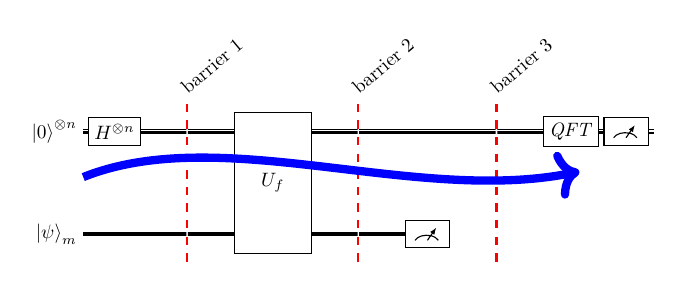
\begin{tikzpicture}[scale=0.7,every label/.style={rotate=40, anchor=south west}]
    \begin{yquant*}[operators/every barrier/.append style={red, thick},
        operator/minimum width=7mm,
        operator/separation=1mm,
        register/separation=10mm]
    qubits {$\ket0^{\otimes n}$} a;
    qubits {$\ket{\psi}_m$} b;
    box {$H^{\otimes n}$} a;
    ["barrier 1"]
    barrier (-);
    [x radius=7mm, y radius=7mm]
    box {$U_f$} (a,b);
    ["barrier 2"]
    barrier (-);
    measure b;
    discard b;
    ["barrier 3"]
    barrier (-);
    box {$\mathit{QFT}$} a;
    measure a;
    \end{yquant*}
    \draw[line width=3pt, ->, blue] (0,-1.1) .. controls (2.5,-0.1) and (6,-1.6) .. (9,-1);
  \end{tikzpicture}
  \caption{Conventional Flow}
  \end{subfigure}
  \begin{subfigure}{0.5\textwidth}
  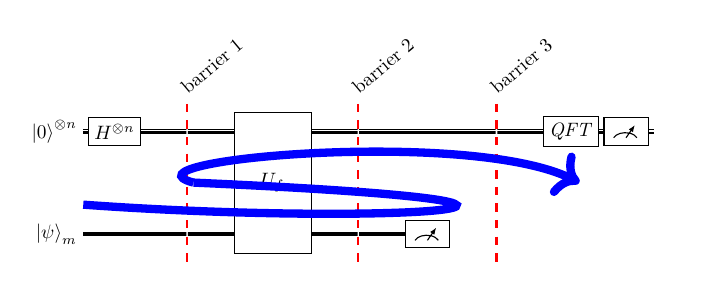
\begin{tikzpicture}[scale=0.7,every label/.style={rotate=40, anchor=south west}]
    \begin{yquant*}[operators/every barrier/.append style={red, thick},
        operator/minimum width=7mm,
        operator/separation=1mm,
        register/separation=10mm]
    qubits {$\ket0^{\otimes n}$} a;
    qubits {$\ket{\psi}_m$} b;
    box {$H^{\otimes n}$} a;
    ["barrier 1"]
    barrier (-);
    [x radius=7mm, y radius=7mm]
    box {$U_f$} (a,b);
    ["barrier 2"]
    barrier (-);
    measure b;
    discard b;
    ["barrier 3"]
    barrier (-);
    box {$\mathit{QFT}$} a;
    measure a;
  \end{yquant*}
  \draw[line width=3pt, blue] (0,-1.6) .. controls (5.5,-2) and (11,-1.6) .. (2,-1.2);
  \draw[line width=3pt, ->, blue] (2,-1.2) .. controls (0.5,-0.8) and (7,-0.2) .. (9,-1.2);
  \end{tikzpicture}
  \caption{\label{fig:retroflow}Retrodictive Flow}
  \end{subfigure}
\caption{\label{fig:templateQC}Template quantum circuit}
\end{figure}

\paragraph*{Template for Circuits.}
All the problems above have solutions using quantum circuits that all
fit the template in Fig.~\ref{fig:templateQC}. The $U_f$ block, often
called the ``oracle'', is uniformly defined as:
\begin{equation}
  U_f(\ket{x}\ket{y}) = \ket{x}\ket{f(x) \oplus y},
\end{equation}
for all the problems. We also use the Quantum Fourier Transform (QFT)
uniformly as the last step in all the circuits although for most
circuits, with the notable exception of Shor's algorithm, the low
precision approximation of QFT (which is the Hadamard gate) is
sufficient~\cite{aqft}. 

After replacing $H\ket{0}$ by a symbolic variable, the $U_f$ block
ends up being completely classical, albeit performing mixed mode
execution of the circuit. More precisely, it means that in all these
algorithms, the top collection of wires (which we will call the
input register) is prepared in a uniform superposition which
can be represented using symbolic variables. The measurement of the
bottom collection of wires (which we call the output register) after
barrier 2 provides partial information about the future which is,
together with the initial conditions of the output register,
sufficient to symbolically execute the circuit. In each case, instead
of the conventional execution flow depicted in
Fig.~\ref{fig:templateQC}(a), we find a possible measurement
outcome~$w$ at barrier (2) and perform a symbolic retrodictive
execution with a state $\ket{xw}$ going backwards to collect the
constraints on $x$ that enable us to solve the problem in question.

\begin{figure}[t]
  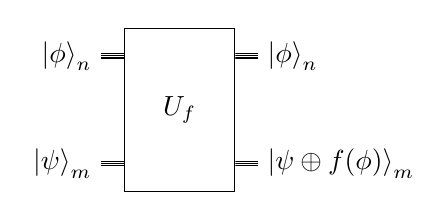
\begin{tikzpicture}[every label/.style={rotate=40, anchor=south west}]
    \begin{yquant*}[
        operator/minimum width=7mm,
        operator/separation=3mm,
        register/separation=10mm]
    qubits {$\ket{\phi}_n$} a;
    qubits {$\ket{\psi}_m$} b;
    [x radius=7mm, y radius=7mm]
    box {$U_f$} (a,b);
    output {$\ket{\phi}_n$} a;
    output {$\ket{\psi \oplus f(\phi)}_m$} b;
    \end{yquant*}
  \end{tikzpicture}
\caption{\label{fig:CircuitAbstraction}Circuit Abstraction}
\end{figure}

In other words, from the perspective of our approach to symbolic
execution, it is possible to disregard the initial Hadamard gates and
the final QFT block and it suffices to look at circuits that match the
template in Fig.~\ref{fig:CircuitAbstraction}.

%%%%%%%%%%%%%%%%%%%%%%%%%%%%%%%%%%%%%%%%%%%%%%%%%%%%%%%%%%%%%%%%%%%%%%%%%
\section{Design and Implementation}
\label{sec4}

Our exposition of the design and implementation of our system will
follow the advice of~\citet{parnas1986rational} on \emph{faking it}:
a reconstruction of the requirements as we should have had them if
we'd been all-knowing, and a design that fits those requirements. The
version history in our GitHub repository can be inspected for anyone
who wants to see our actual path.

As we experimented with the idea of partial evaluation and symbolic
execution of quantum circuits, we ended up writing a lot of variants of
essentially the same code, but with minor differences in representation.
From these early experiments, we could see the major variation points:
\begin{itemize}
  \item representation of \emph{boolean values} and \emph{boolean functions},
  \item representation of ANF,
  \item representation of circuits.
\end{itemize}
We also wanted to write out circuits only once, and have them be valid
across these representation changes and be executable forwards,
backwards, and mixed retrodictive mode.

With the notable exception of Shor's algorithm, all the algorithms we
study are expressed in the ``black-box model.'' In that model, the
circuit implementing the $U_f$ is collapsed to just one function
call. Of course, in any actual use of the algorithm, this circuit must
be implemented and its execution time must be accounted
for. Therefore, we want to---offline--- synthesize a circuit from the
boolean specification, i.e., for $f : \Bool^n \rightarrow\Bool$, we
wish to generate the circuit for
$g : \Bool^{n+1} \rightarrow \Bool^{n+1}$ such that for
$\overline{x} : \Bool^n$ we have
$g(\overline{x},y) = (\overline{x}, y \oplus f(\overline{x}))$.

This leads us to the following requirements that our code must
fulfill.

\begin{figure*}[t]
\begin{tabular}{l | p{13cm}}
  \textbf{Module} & \textbf{Service} \\ \hline
  \texttt{Value} & representation of a \emph{language of values}
    (as a typeclass) and some constructors\\
  \texttt{VarInFormula} & abstract representation of variables in formulae\\
  \texttt{Variable} & variables as locations holding values and
    their constructors\\
  \texttt{ModularArith} & modular arithmetic utilities useful in
    implementing certain algorithms, like Shor's\\
  \texttt{BoolUtils} & function to interpret a list of booleans as
    an Integer\\
  \texttt{GToffoli} & representation of generalized Toffoli gates
    and some constructors\\
  \texttt{Circuits} & representation of circuits (sequences of gates)
    and of the special ``wires'' of our circuits\\
  \texttt{Synthesis} & synthesis algorithm for circuits with particular
    properties\\
  \texttt{ArithCirc} & creation of arithmetic circuits\\
  \texttt{EvalZ} & evaluation of circuits on concrete values\\
  \texttt{FormAsList} & representation of formulae as xor-lists
    of and-lists of literals-as-strings\\
  \texttt{FormAsMaps} & representation of formulae as xor-maps
    of and-maps of literals-as-Int\\
  \texttt{FormAsBitmaps} & representation of formulae as xor-maps
    of bitmaps\\
  \texttt{SymbEval} & Symbolic evaluation of circuits\\
  \texttt{SymbEvalSpecialized} & Symbolic evaluation of circuits
    specialized to the representation from \texttt{FormAsBitmaps}\\
  \texttt{QAlgos} & generating the circuits themselves\\
  \texttt{RunQAlgos} & running the actual circuits \\
  \texttt{Trace} & utilities for tracing and debugging
\end{tabular}
  \caption{Modules and their services}
  \label{fig:modules}
\end{figure*}

\subsection{Requirements}

We need to be able to deal with the following variabilities:
\begin{enumerate}
  \item multiple representations of \emph{boolean values},
  \item multiple representations of \emph{boolean formulae},
  \item different evaluation means (directly, symbolically, forwards,
    backwards, retrodictive),
\end{enumerate}

\noindent It must also be possible to implement the following:
\begin{enumerate}[resume]
  \item a reusable representation of circuits composed of generalized Toffoli gates,
  \item a reusable representation of the inputs, outputs and ancillae associated to
    a circuit,
  \item a \emph{synthesis} algorithm for circuits implementing a certain boolean
    function,
  \item a reusable library of circuits (such as
    Deutsch, Deutsch-Jozsa, Bernstein-Vazirani, Simon, Grover, and Shor).
\end{enumerate}
\noindent From those, we can make a
set of design choices that drive the eventual solution.

We eventually want some non-functional characteristics to hold:
\begin{enumerate}[resume]
  \item evaluation of reasonably-sized circuits should be relatively efficient.
\end{enumerate}

\subsection{Design}

To meet the first requirement, we use \emph{finally tagless}~\cite{tagless}
to encode a \emph{language of values}:
\begin{minted}{haskell}
  class (Show v, Enum v) => Value v where
  zero :: v
  one  :: v
  snot :: v -> v
  sand :: v -> v -> v
  sxor :: v -> v -> v

  -- has a default implementation
  snand :: [v] -> v -- n-ary and
  snand = foldr sand one
\end{minted}
\noindent which is then implemented $4$ times, once for $\texttt{Bool}$
and then multiple times for different symbolic variations. As a side-effect,
this gives us requirement $3$ ``for free'' if we can write a sufficiently
polymorphic evaluator (which we will present below).

Unlike value representations that can be computed from context, we
want to explicitly choose how to represent variables in formulas
ourselves (part of requirement 2).  Thus we use an explicit record instead of an
implicit dictionary:

\begin{minted}{haskell}
data VarInFormula f v = FR
  { fromVar  :: v -> f
  , fromVars :: Int -> v -> [ f ]
  }
\end{minted}
Each formula representation may have different
\emph{variable representation} \texttt{v}
and how to insert them into the current \emph{formula representation} \texttt{f},
singly or as $n$ formulas.

A generalized Toffoli gate can be represented by a list of representation of
value accessors \texttt{br} (short for boolean representation) along with a list
of \emph{controls} that tell us whether to use the bit directly or negated,
along with which value will potentially be flipped. The implementation of very
common gates (negation and controlled not) are also shown.
\begin{minted}{haskell}
data GToffoli br = GToffoli [Bool] [br] br

xop :: br -> GToffoli br
xop = GToffoli [] []

cx :: br -> br -> GToffoli br
cx a = GToffoli [True] [a]
\end{minted}
\noindent The core of a circuit (requirement $4$) is then implemented as a
sequence of these (where \texttt{Seq} is from {Data.Sequence}).
\begin{minted}{haskell}
type OP br = Seq (GToffoli br)
\end{minted}

\noindent Mainly for efficiency reasons, we model circuits as manipulating
\emph{locations holding values} rather than directly acting on values. We
use \texttt{STRef}s (aliased to \texttt{Var}) for that purpose. Putting this
together with the circuit template of \ref{sec3}, we get
\begin{minted}{haskell}
data Circuit s v = Circuit
  { op          :: OP (Var s v)
  , xs          :: [Var s v]
  , ancillaIns  :: [Var s v]
  , ancillaOuts :: [Var s v]
  , ancillaVals :: [v]
  }
\end{minted}
\noindent which lets us achieve requirement $5$.

For requirement $6$, we implement a straightforward version of a
well-established algorithm~\cite{soeken2016fast}. Our implementation
is \emph{language agnostic}, in other words it works via the
\texttt{Value} interface, so that the resulting circuits are all of
type \texttt{OP br} for a free representation \texttt{br}. As circuit
synthesis is only done for generating examples, we are not worried
about its efficiency.

The arithmetic circuit generators are also based on textbook algorithms, and are
not optimized in any way, neither for running time nor for gate count. Neither are
the code for the quantum algorithms. They are, however, representation
polymorphic.

Above, we said we had $3$ different symbolic evaluators. These were not driven
by having different levels of \emph{precision} but rather by requirement $8$,
efficiency. Our first evaluator (\texttt{FormAsList}) uses xor-lists of
and-lists of literals (as strings, i.e.,
\texttt{"x0"}, \texttt{"x1"}, \ldots in lexicographical order of the wires). ANF
is then easy: and-lists are sorted, and duplicates removed. Xor-lists are sorted,
grouped, even length lists are removed, and then made unique. This is woefully
inefficient, and was the clear bottleneck in our profiles.

A less na\"{\i}ve approach uses a set of bits for representing literals, an
\texttt{IntSet} for and-lists, and a normalized multiset for xor maps (a normalized
multiset is one with only $0$ and $1$ as multiplicities). We found
it more efficient to use a multiset for intermediate computations with xor maps
which is normalized at the end instead of trying to track even/odd number of
occurrences. Only computing Cartesian products in this representation requires
some thought for finding a reasonably efficient algorithm.

While significantly faster, this representation still did not make our programs
sufficiently efficient. Our final representation uses natural numbers as
and-maps where the encoding of literals is now positional, and xor maps are
again multisets of these ``bitmaps.''

As a last optimization, our circuits have a very particular property: the control
wires are not written to, so that they are all literals. We use this
further optimize the evaluation of single gates.

\subsection{Implementation}

The final code consists of $18$ modules that implement various
services, see Fig.~\ref{fig:modules} for a full listing. It consists of
only $1449$ lines of Haskell text, of which $646$ lines are blank, import or
comments, module declaration, so that $809$ are ``code.'' Testing and printing
utilities are not counted in the above.

The code that occupies the most volume is that for running the examples, as each
circuit needs its own setup for the input and output wires. Next is the implementation
of symbolic representations of formulae in ANF. This is largely because there are a
lot of pieces that need to be defined, including many instances; the algorithmic aspect
rarely span more than $15$ lines in total. The code for generating arithmetic circuits
is voluminous as well as largely computational, but is a re-implementation of known
material, as is the synthesis code.

A few comments on further implementation details. Sharp readers might have noticed
\texttt{snand} as defined in class \texttt{Value} instead of as a polymorphic function
outside the class; we do this to enable its implementation to be overridden.
Lastly, \texttt{GToffoli}'s implementation relies on an unexpressed invariant: that its
two lists are of equal length. We really ought to refactor the code to use a single
list of tuples, but this is a pervasive change that would not bring much benefit as
we use combinators to build circuits, and these already maintain that invariant.
Similarly for \texttt{Circuit}: the lists \texttt{ancillaIns}, \texttt{ancillaOut}
and \texttt{ancillaVals} should all be of the same length. That invariant is not
checked in our code.

%%%%%%%%%%%%%%%%%%%%%%%%%%%%%%%%%%%%%%%%%%%%%%%%%%%%%%%%%%%%%%%%%%%%%%%%%
\section{Evaluation}
\label{sec5}

We want to evaluate the \emph{effectiveness} of our evaluator by running it
on standard algorithms, as well as its (relative) \emph{efficiency}.

We first give interesting aspects of running the six quantum algorithms
outlined in Sec.~\ref{sec5}, before commenting on complexity and workflow.

\subsection{Symbolic execution of the Algorithms}

Most of the algorithms end up generating differently shaped constraint
systems, and thus each need to be examined on its own. It is worth
noting that all these algorithms are not known to have fast classical
versions except for a few special cases~\cite{calude,djdeq}. We spend more
time on the analysis of Shor's algorithm, as it is both more important
and displays subtle behavior.

\paragraph*{Deutsch and Deutsch-Jozsa.}
We perform a retrodictive execution of the $U_f$ block with an output
measurement~$0$, i.e., with the state $\ket{x_{n-1}\cdots x_1x_00}$.
The result of the execution is a symbolic formula $r$ that determines
the conditions under which $f(x_{n-1},\cdots,x_0) = 0$. When the
function is constant, the results are $0=0$ (always) or $1=0$ (never)
\emph{regardless of how large the circuit is}. When the function is
balanced, we get a formula that mentions the relevant variables. As
examples, we generated all 12872 functions
$\finset{2^6} \rightarrow \finset{2}$ that are valid inputs to the
algorithm; the 2 constant functions and the 12870 balanced functions
at that type. The result of the symbolic execution immediately
provides the answer but with the understanding that the generation of
the formulae takes time depending on the distribution of zeros and
ones. For example, here are the results of three executions for
balanced functions $\finset{2^6} \rightarrow \finset{2}$:
\begin{itemize}
\item $x_0 = 0$,
\item $x_0 \oplus x_1 \oplus x_2 \oplus x_3 \oplus
    x_4 \oplus x_5 = 0$, and
\item $1 \oplus x_3x_5 \oplus x_2x_4 \oplus x_1x_5
\oplus x_0x_3 \oplus x_0x_2 \oplus x_3x_4x_5 \oplus x_2x_3x_5 \oplus
x_1x_3x_5 \oplus x_0x_3x_5 \oplus x_0x_1x_4 \oplus x_0x_1x_2 \oplus
x_2x_3x_4x_5 \oplus x_1x_3x_4x_5 \oplus x_1x_2x_4x_5 \oplus
x_1x_2x_3x_5 \oplus x_0x_3x_4x_5 \oplus x_0x_2x_4x_5 \oplus
x_0x_2x_3x_5 \oplus x_0x_1x_4x_5 \oplus x_0x_1x_3x_5 \oplus
x_0x_1x_3x_4 \oplus x_0x_1x_2x_4 \oplus x_0x_1x_2x_4x_5 \oplus
x_0x_1x_2x_3x_5 \oplus x_0x_1x_2x_3x_4 = 0$.
\end{itemize}
In the first case, the function is balanced because it produces~$0$
exactly when $x_0=0$ which happens half of the time in all possible
inputs; in the second case the output of the function is the
exclusive-or of all the input variables which is another easy instance
of a balanced function. The last case is a cryptographically strong
balanced function whose output pattern is balanced but, by design,
difficult to discern~\cite{quteprints21763}.

\begin{insight} In these algorithms, we actually do not care about the
  exact formula. Indeed, since we are \emph{promised} that the
  function is either constant or balanced, then any formula that
  refers to at least one variable must indicate a balanced function:
  the outcome of the algorithm can be immediately decided if the
  formula is anything other than 0 or 1.  Since the symbolic
  evaluation executes the $U_f$ block ``once,'' one might conclude
  that it is a ``de-quantization'' of the algorithm in the black-box
  model, producing immediate answers even in cases when the quantum
  algorithm generates complicated entangled patterns during quantum
  evolution~\cite{djdeq}. However, it is important to remember that
  our circuits are ``white-box'' rather than ``black-box'' and that
  the time taken to execute the circuit is part of the overall
  complexity of the algorithm. We defer to Sec.~\ref{sub:complexity}
  for a more detailed discussion of this point and refer to
  \citet{10.1145/3341106} for another perspective on black-box
  vs. white-box complexity in the context of graph algorithms.
\end{insight}

\begin{signif}
  That the details of the equations do not matter is crucial as the
  satisfiability of generally boolean equation is, in general, an
  $\mathit{NP}$-complete
  problem~\cite{4640789,Karp1972,10.1145/800157.805047}. More
  directly, the answer to the algorithm does \emph{not} require an
  exact calculation of the pre-image of the boolean function. Indeed,
  based on the conjectured existence of one-way functions which itself
  implies $\mathit{P} \neq \mathit{NP}$, pre-images calculations are
  believed to be computationally intractable in their most general
  setting.  What is intriguing is that quantum algorithms appear to be
  able to answer certain general queries about pre-images without
  explicitly calculating the pre-image.
\end{signif}

\paragraph*{Bernstein-Vazirani.}
We show a complete small example. Let $n=8$ and let the secret string
$s = 00111010$. In this case, the problem becomes: given a circuit for
$f(x) = x_1 \oplus x_3 \oplus x_4 \oplus x_5$, determine the secret
string. There are naturally many circuits that realize the function
$f$; in our ``white-box'' model the running time of the symbolic
execution will depend on which circuit is given. In the example below,
we generate the simplest circuit: as all equivalent circuit have the
same ANF representation, any other circuit would give the same
symbolic output but potentially taking longer to execute:

\begin{minted}{haskell}
retroBernsteinVazirani fr = print $ runST $ do                                    
  xs <- newVars (fromVars fr 8 "x")                                               
  y <- newVar zero                                                                
  let op = fromList [ cx (xs !! 1) y                                              
                    , cx (xs !! 3) y                                              
                    , cx (xs !! 4) y                                              
                    , cx (xs !! 5) y                                              
                    ]                                                             
  run Circuit { op = op                                                           
              , xs = xs                                                           
              , ancillaIns = [y]                                                  
              , ancillaOuts = [y]                                                 
              , ancillaVals = undefined                                           
              }                                                                   
  readSTRef y                                                                     
                                                                                  
runRetroBernsteinVazirani :: IO ()                                                
runRetroBernsteinVazirani = 
  retroBernsteinVazirani FL.formRepr                    
                            
-- > runRetroBernsteinVazirani 
-- x_1 \oplus x_3 \oplus x_4 \oplus x_5
\end{minted}
As can be seen, \h{retroBernsteinVazirani} is parameterized by a
representation of formulae: it allocates 8 symbolic variables,
initializes the output to \h{zero}, generates the circuit, and runs
it. The top level call \h{runRetroBernsteinVazirani} just needs to
pick a particular representation of formulae. The result is the ANF
representation of the circuit, from which the secret string can be
read off: the indices $\{1,3,4,5\}$ are the indices at which the secret
string is 1.

\begin{insight}
  Generally, the formulae are guaranteed to be of the form
  $\sum_i x_i$ for some indices $i$; the secret string is then the
  binary number that has a 1 at those indices.
\end{insight}

\paragraph*{Simon.}
The circuit below implements the black box for a function $f$ such
that $f(0) = f(3) = 0$ and $f(1) = f(2) = 3$:
\begin{center}
\begin{quantikz}\label{eq:simon}
   \lstick{$x_0$} & \ctrl{2} & \ctrl{3} & \qw      & \qw      & \rstick{$x_0$} \qw \\
   \lstick{$x_1$} & \qw      & \qw      & \ctrl{1} & \ctrl{2} & \rstick{$x_1$} \qw \\
   \lstick{$a_0$} & \targ{}  & \qw      & \targ{}  & \qw      & \rstick{$a_0$} \qw \\
   \lstick{$a_1$} & \qw      & \targ{}  & \qw      & \targ{}  & \rstick{$a_1$} \qw
\end{quantikz}
\end{center}

\noindent We have for all $x \in [0..3]$ that $f(x) = f(x \oplus 3)$
where $\oplus$ is applied bitwise, i.e., the secret value $a=3$. To
extract this~$a$ via symbolic execution we proceed as follows. We
first pick a random $x$, say $x = 3$, fix the initial condition
$a = 0$ and run the circuit forward. This execution produces, in the
output register, the value of $f(x) = 0$. We now run a symbolic
retrodictive execution with $a = 0$ at the output site. That execution
produces information on all values of $a$ that are consistent with the
observed result. In this case, we get: $a_0 = x_0 \oplus x_1$ and
$a_1 = x_0 \oplus x_1$. Reconciling these equations with the initial
conditions $a_0=a_1=0$, we conclude $x_0=x_1$. In other words, any
input $x_1x_0$ such that $x_0=x_1$ is consistent with the observed
result. There are two such inputs $x=0$ or $x=3$ and the secret $a$ is
their difference. 

\begin{insight}
  Simon's problem does not seem to have a resolution that is easy to read
  from the resulting equations. Generally, we get equations that have
  exactly two solutions, one of which is known. In some cases, like
  above, it is straightforward to infer the second solution, but as
  the equations get more and more complex, the problem becomes
  harder. 
\end{insight}

\begin{figure*}[t]
\begin{tabular}{ll}
$u=0$ &
  $\red{1} \oplus x_3 \oplus x_2 \oplus x_1 \oplus x_0 \oplus x_2x_3 \oplus x_1x_3 \oplus x_1x_2 \oplus x_0x_3 \oplus x_0x_2 \oplus x_0x_1 \oplus x_1x_2x_3 \oplus x_0x_2x_3$ \\
   &\quad $\oplus ~x_0x_1x_3 \oplus x_0x_1x_2 \oplus x_0x_1x_2x_3$ \\
$u=1$ &
  $\red{x_0} \oplus x_0x_3 \oplus x_0x_2 \oplus x_0x_1 \oplus x_0x_2x_3 \oplus x_0x_1x_3 \oplus x_0x_1x_2 \oplus x_0x_1x_2x_3$ \\
$u=2$ &
  $\red{x_1} \oplus x_1x_3 \oplus x_1x_2 \oplus x_0x_1 \oplus x_1x_2x_3 \oplus x_0x_1x_3 \oplus x_0x_1x_2 \oplus x_0x_1x_2x_3$ \\
$u=3$ &
  $\red{x_0x_1} \oplus x_0x_1x_3 \oplus x_0x_1x_2 \oplus x_0x_1x_2x_3$ \\
$u=4$ &
  $\red{x_2} \oplus x_2x_3 \oplus x_1x_2 \oplus x_0x_2 \oplus x_1x_2x_3 \oplus x_0x_2x_3 \oplus x_0x_1x_2 \oplus x_0x_1x_2x_3$ \\
$u=5$ &
  $\red{x_0x_2} \oplus x_0x_2x_3 \oplus x_0x_1x_2 \oplus x_0x_1x_2x_3$ \\
$u=6$ &
  $\red{x_1x_2} \oplus x_1x_2x_3 \oplus x_0x_1x_2 \oplus x_0x_1x_2x_3$ \\
$u=7$ &
  $\red{x_0x_1x_2} \oplus x_0x_1x_2x_3$ \\
$u=8$ &
  $\red{x_3} \oplus x_2x_3 \oplus x_1x_3 \oplus x_0x_3 \oplus x_1x_2x_3 \oplus x_0x_2x_3 \oplus x_0x_1x_3 \oplus x_0x_1x_2x_3$ \\
$u=9$ &
  $\red{x_0x_3} \oplus x_0x_2x_3 \oplus x_0x_1x_3 \oplus x_0x_1x_2x_3$ \\
$u=10$ &
  $\red{x_1x_3} \oplus x_1x_2x_3 \oplus x_0x_1x_3 \oplus x_0x_1x_2x_3$ \\
$u=11$ &
  $\red{x_0x_1x_3} \oplus x_0x_1x_2x_3$ \\
$u=12$ &
  $\red{x_2x_3} \oplus x_1x_2x_3 \oplus x_0x_2x_3 \oplus x_0x_1x_2x_3$ \\
$u=13$ &
  $\red{x_0x_2x_3} \oplus x_0x_1x_2x_3$ \\
$u=14$ &
  $\red{x_1x_2x_3} \oplus x_0x_1x_2x_3$ \\
$u=15$ &
  $\red{x_0x_1x_2x_3}$
\end{tabular}
\caption{\label{fig:Grover}Result of retrodictive execution for the Grover oracle ($n=4$, $w$ in the range $\{0..15\}$). The highlighted red subformula is the binary representation of the hidden input $u$.}
\end{figure*}

\paragraph*{Grover.}
A reversible oracle circuit for a function $f(x)$ that returns 1 for a
unique input $u$ and 0 otherwise is rather trivial: it consists of a
single generalized Toffoli gate that flips the output when the input
matches $u$:
\begin{minted}{haskell}
synthesisGrover :: 
  Int -> [Var s v] -> Integer -> OP s v
synthesisGrover n (viewL -> (xs,y)) u =
  S.singleton $ GToffoli (fromInt n u) xs y
\end{minted}
The ANF representation of the circuit is sensitive to the value
$u$ as shown in Fig.~\ref{fig:Grover} and the running time of symbolic
execution varies accordingly. What is interesting is that the shortest
subformula in the ANF representation is guaranteed to be the binary
representation of $u$. As an example, if $u=3$, then
$x_1x_0$ must be a subformula in the ANF representation. By itself,
this subformula would satisfy not just 3 but also 7, 11, and 15.  To
exclude this latter values, the ANF representation includes the clause
$x_2x_1x_0$ to exclude 7, the formula $x_3x_1x_0$ to exclude 11, and
the formula $x_3x_2x_1x_0$ to exclude~15. 

\begin{insight}
  For Grover as well, the result can be immediately read off the formula.
\end{insight}

\begin{figure}
\begin{center}
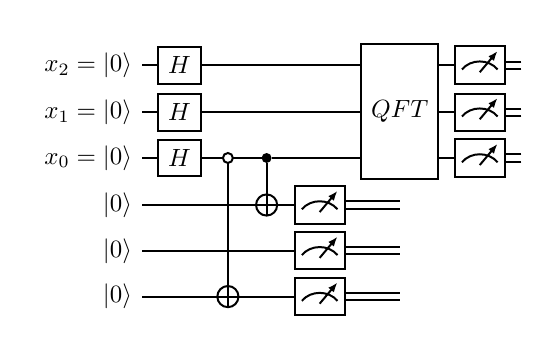
\begin{tikzpicture}
\node[scale=0.9]{
\begin{quantikz}[row sep=0.005cm,column sep=0.22cm]
\lstick{$x_2 = \ket{0}$} & \gate{H}& \qw & \qw
      & \qw & \gate[wires=3][0.5cm]{QFT} & \meter{} & \cw \\
\lstick{$x_1 = \ket{0}$} & \gate{H} & \qw & \qw
      & \qw & & \meter{} & \cw \\
\lstick{$x_0 = \ket{0}$} & \gate{H} & \octrl{3} & \ctrl{1}
      & \qw & & \meter{} & \cw \\
\lstick{$\ket{0}$} & \qw & \qw & \targ{}
      & \meter{} & \cw \\
\lstick{$\ket{0}$} & \qw & \qw  & \qw
      & \meter{} & \cw \\
\lstick{$\ket{0}$} & \qw & \targ{} & \qw
      & \meter{} & \cw
\end{quantikz}
};\end{tikzpicture}
\end{center}
\caption{\label{fig:shor15}Finding the period of $4^x \mod{15}$}
\end{figure}
\begin{figure*}
\[\begin{array}{l@{\quad}lllll}
\textrm{Base} & \multicolumn{4}{c}{\textrm{Equations}} & \textrm{Solution} \\[2ex]
a=11 & x_0 = 0 &&&& \red{x_0 = 0} \\
a=4,14 & 1 \oplus x_0 = 1 & x_0 = 0 &&
  & \red{x_0 = 0} \\
a=7,13 & 1 \oplus x_1 \oplus x_0x_1 = 1 & x_0x_1 = 0 & x_0 \oplus x_1 \oplus x_0x_1 = 0 &  x_0 \oplus x_0x_1 = 0 & \red{x_0=x_1=0} \\
a=2,8 & 1 \oplus x_0 \oplus x_1 \oplus x_0x_1 = 1 & x_0x_1 = 0 & x_1 \oplus x_0x_1 = 0 & x_0 \oplus x_0x_1 = 0  & \red{x_0=x_1=0}
\end{array}\]
\caption{\label{fig:shor-eqs}Equations generated by retrodictive
  execution of $a^x \mod{15}$ for different values of $a$, starting
  from observed result 1 and unknown
  $x_8x_7x_6x_5x_4x_3x_2x_1x_0$. The solution for the unknown
  variables is given in the last column.}
\end{figure*}

\paragraph*{Shor.}
The circuit in Fig.~\ref{fig:shor15} uses a hand-optimized
implementation of quantum oracle $U_f$ for the modular exponentiation
function $f(x) = 4^x \mod{15}$ to factor 15 using Shor's algorithm.
In a conventional forward execution, the state before the QFT block
is:
\[
\frac{1}{2\sqrt{2}} (
  (\ket{0} + \ket{2} + \ket{4} + \ket{6}) \ket{1} +
  (\ket{1} + \ket{3} + \ket{5} + \ket{7}) \ket{4}
  ) .
\]
At this point, the output register is measured to be either $\ket{1}$ or
$\ket{4}$. In either case, the input register snaps to a state
of the form $\sum_{r=0}^3 \ket{a+2r}$ whose QFT has peaks at $\ket{0}$
or~$\ket{4}$ making them the most likely outcomes of measurements of
the input register. If we measure $\ket{0}$, we repeat the
experiment; otherwise we infer that the period is~2.

In the backwards execution, we can start with the state
$\ket{x_2x_1x_0001}$ since 1 is guaranteed to be a possible output
measurement (corresponding to $f(0)$). The first \cx-gate changes the
state to $\ket{x_2x_1x_0x_001}$ and the second \cx-gate produces
$\ket{x_2x_1x_0x_00x_0}$. At that point, we reconcile the retrodictive
result of the output register $\ket{x_00x_0}$ with the initial
condition $\ket{000}$ to conclude that $x_0=0$. In other words, in
order to observe the output at $001$, the input register must
be initialized to a superposition of the form $\ket{??0}$ where the
least significant bit must be 0 and the other two bits are
unconstrained. Expanding the possibilities, the input register needs
to be in a superposition of the states
$\ket{000}, \ket{010}, \ket{100}$ or $\ket{110}$ and we have just
inferred using purely classical but retrodictive reasoning that the
period is 2.

This result does not, in fact, require the small optimized circuit of
Fig.~\ref{fig:shor15}. In our implementation, modular exponentiation
circuits are constructed from first principles using adders and
multipliers~\cite{PhysRevA.54.147}. In the case of $f(x) = 4^x
\mod{15}$, although the unoptimized constructed circuit has 56,538
generalized Toffoli gates,
the execution results in just two simple equations: $x_0 = 0$ and $1
\oplus x_0 = 1$. Furthermore, as shown in Fig.~\ref{fig:shor-eqs}, the
shape and size of the equations is largely insensitive to the choice
of 4 as the base of the exponent, leading in all cases to the
immediate conclusion that the period is either 2 or 4. When the
solution is $x_0=0$, the period is 2, and when it is $x_0=x_1=0$, the
period is~4.

The remarkable effectiveness of retrodictive computation of the Shor
instance for factoring 15 is due to a coincidence: a period that is a
power of 2 is clearly trivial to represent in the binary number system
which, after all is expressly designed for that purpose. That
coincidence repeats itself when factoring products of the (known)
Fermat primes: 3, 5, 17, 257, and 65537, and leads to small
circuits~\cite{shorFermat}. This is confirmed with our implementation
which smoothly deals with unoptimized circuits for factoring such
products. Factoring 3*17=51 using the unoptimized circuit of 177,450
generalized Toffoli gates produces just the 4 equations: $1 \oplus x_1
= 1$, $x_0 = 0$, $x_0 \oplus x_0x_1 = 0$, and $x_1 \oplus x_0x_1 =
0$. Even for 3*65537=196611 whose circuit has 4,328,778 generalized
Toffoli gates, the execution produces 16 small equations that refer to
just the four variables $x_0$, $x_1$, $x_2$, and $x_3$ constraining
them to be all 0, i.e., asserting that the period is 16.

\begin{figure}
  \centering
    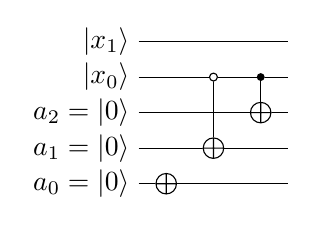
\begin{tikzpicture}[scale=1.0]
   \begin{yquant*}
   qubit {$\ket{x_1}$} x1;
   qubit {$\ket{x_0}$} x0;
   qubit {$a_2 = \ket0$} a2;
   qubit {$a_1 = \ket0$} a1;
   qubit {$a_0 = \ket0$} a0;
   not a0;
   align -;
   cnot a1 | ~x0;
   cnot a2 | x0;
  \end{yquant*}
\end{tikzpicture}
\caption{\label{fig:shor21}Finding the period of $4^x \mod{21}$ using
  qutrits. The three gates are from left to right are the $X$,
  $\textrm{SUM}$, and $C(X)$ gates for ternary
  arithmetic~\cite{10.5555/3179473.3179481}. The $X$ gate adds 1
  modulo 3; the controlled version $C(X)$ only increments when the
  control is equal to 2, and the \textrm{SUM} gates maps $\ket{a,b}$
  to $\ket{a,a+b}$.}
\end{figure}
Since periods that are powers of 2 are rare and special, we turn our
attention to factoring problems with other periods. The simplest such
problem is that of factoring 21 with an underlying function
$f(x) = 4^x \mod{21}$ of period 3. The unoptimized circuit constructed
from the first principles has 78,600 generalized Toffoli gates; its
execution generates just three equations. But even in this rather
trivial situation, the equations span 5 pages of text!  A small
optimization reducing the number of qubits results in a circuit of
15,624 generalized Toffoli gates whose execution produces still quite
large, but more reasonable, equations. To understand the reason for
these unwieldy equations, we examine a general ANF formula of the form
$ X_1 \oplus X_2 \oplus X_3 \oplus \ldots = 0$ where each $X_i$ is a
conjunction of some boolean variables, i.e., the variables in each $X$
exhibit constructive interference as they must all be true to enable
that $X=1$. Since the entire formula must equal to 0, every $X_i = 1$
must be offset by another $X_j = 1$, thus exhibiting negative
interference among $X_i$ and~$X_j$. Generally speaking, arbitrary
interference patterns can be encoded in the formulae at the cost of
making the size of the formulae exponential in the number of
variables. This exponential blowup is actually a necessary condition
for any quantum algorithm that can offer an exponential speed-up over
classical computation~\cite{10.2307/3560059}.

It would however be incorrect to conclude that factoring 21 is
inherently harder than factoring 15. The issue is simply that the
binary number system is well-tuned to expressing patterns over powers
of 2 but a very poor match for expressing patterns over powers of
3. Indeed, we show that by just using qutrits, the circuit and
equations for factoring 21 become trivial while those for factoring 15
become unwieldy. The manually optimized circuit in
Fig.~\ref{fig:shor21} consists of just three gates; its retrodictive
execution produces two equations: $x_0=0$ and $x_0 \neq 2$, setting
$x_0=0$ and leaving $x_1$ unconstrained. The matching values in the
qutrit system as 00, 10, 20 or in decimal 0, 3, 6 clearly identifying
the period to be 3. 

\subsection{Time Measurements}

\begin{figure}
 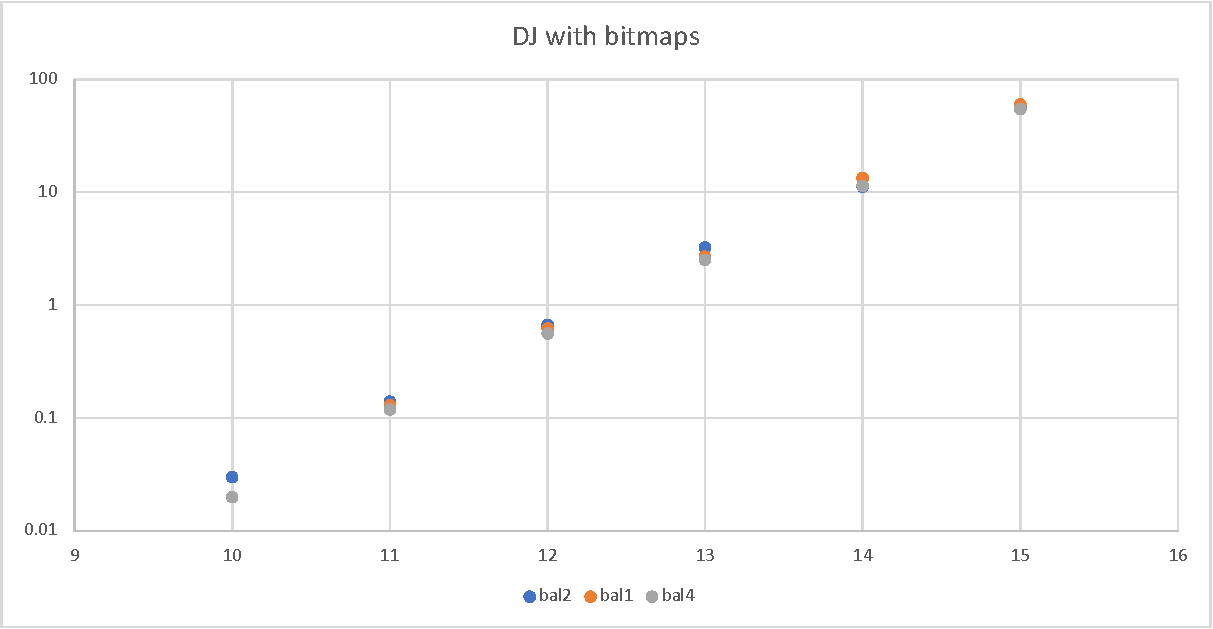
\includegraphics[scale=0.4]{../execution/RetroPE/DJ.pdf}
  \caption{\label{fig:DJ} Deutsch-Jozsa on $3$ problems at different sizes}
\end{figure}

\begin{figure}
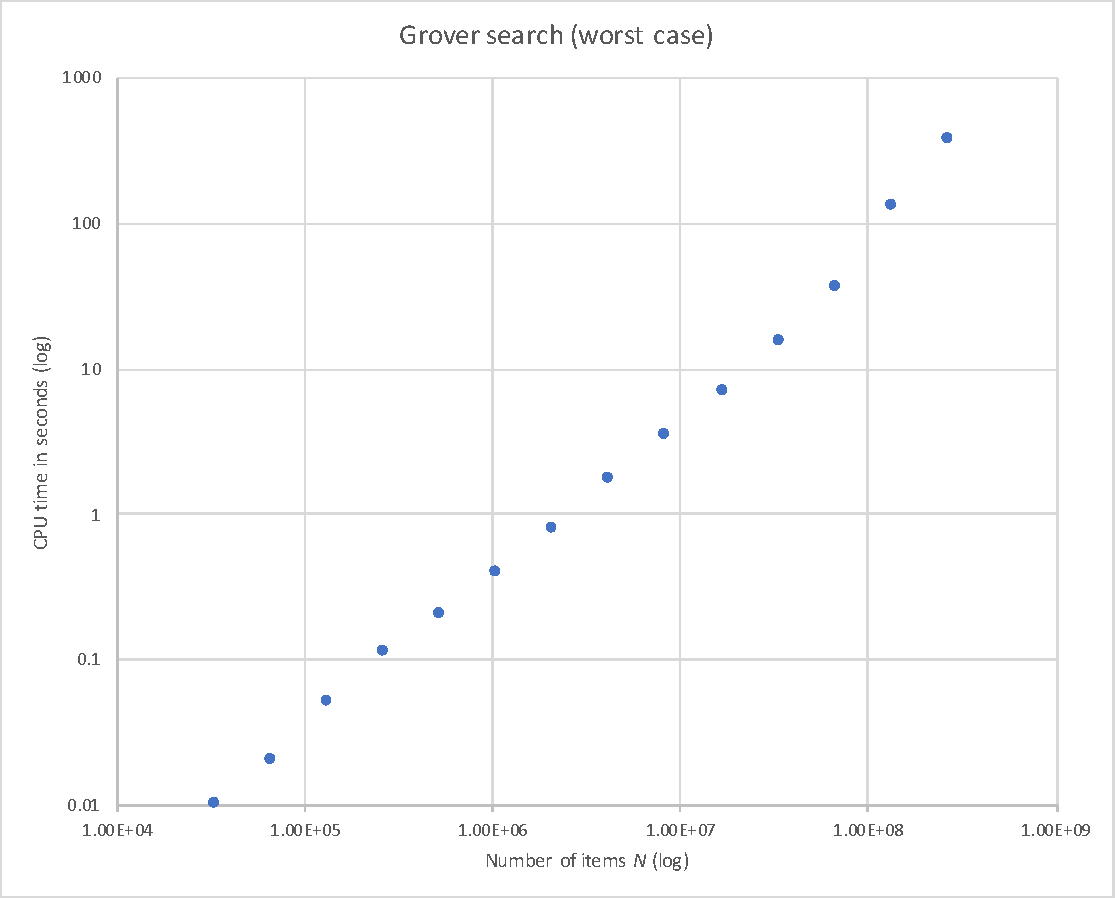
\includegraphics[scale=0.4]{../execution/RetroPE/grover.pdf}
  \caption{\label{fig:GroverWC} Grover on different ``secret'' values $u$ at different sizes}
\end{figure}

\begin{figure}
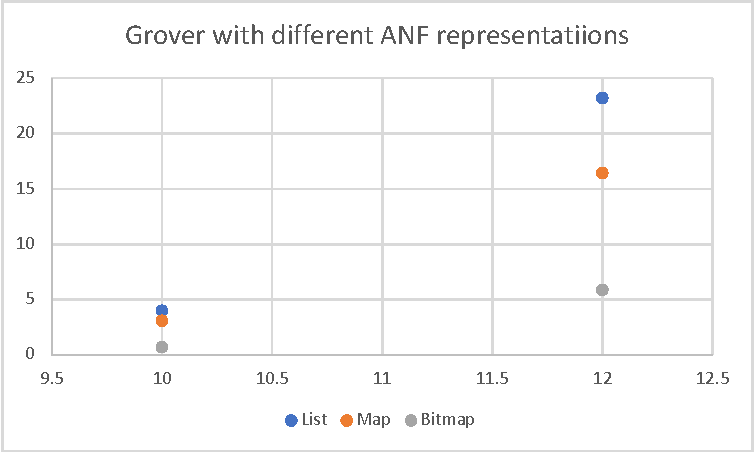
\includegraphics[scale=0.6]{../execution/RetroPE/Grover1.pdf}
  \caption{\label{fig:GroverImpl} Grover at $2$ sizes but using different ANF representations on $u=0$}
\end{figure}

We show a few representative set of timings for the Deutsch-Jozsa and
Grover problems.

Fig.~\ref{fig:DJ} shows what happens when we vary the
size of the problem for Deutsch-Josza on three different balanced
functions: \texttt{bal1} is $x_0$, \texttt{bal2} is $x0\oplus\ldots\oplus x_n$
and \texttt{bal4} is $x_n$. All three show
clear exponential behavior that does not depend on the size of the final
answer. We show the timings only for a single implementation of the
representation of formulae as, somewhat mysteriously, this makes no
difference in this case, we get essentially the same result in all cases.

Fig.~\ref{fig:GroverWC} shows timings of different calls to Grover's
algorithm, using the best representation for formulae (as bitmaps) but varying
what ``secret value $u$'' we are looking for. Here
the binary representation of $u$ matters greatly, ranging from what looks
like essentially constant time to exponential time.

Lastly, Fig.~\ref{fig:GroverImpl} shows Grover's algorithm again, using the
worst case value from the previous figure ($u=0$) but varying the representation
at two sizes. Here we can clearly see the very strong effect that this has
on the timings. This is not just a constant improvement, it is also a complexity
improvement.

\subsection{Complexity}
\label{sub:complexity}

In the general case, we have a circuit containing $T$ generalized
Toffoli gates over $n+m$ qubits split in two registers $A$ ($n$
qubits) and $B$ (m qubits). The typical symbolic execution takes the
following steps with the given worst-case complexity:

\begin{enumerate}
\item If the quantum algorithm is expressed in terms of calls to a
  black-box oracle (all the problems we consider except Shor), then
  the first step is to design the oracle \emph{efficiently}. Perhaps
  surprisingly, it turns out we don’t have to be particularly clever
  in designing that circuit: textbook designs with million of gates
  can work well.
  \item Let $A = \ket{00\ldots 0}$ and $B = \ket{00\ldots 0}$ and run the
circuit with classical inputs. This has complexity $\mathcal{O}(T)$ as
it takes $T$ steps where each step takes constant time. The result of
this evaluation will leave $A$ intact and produce some value $b$ for
the $B$ register.
\item We now run the circuit backwards with the symbolic
values $A = \ket{x_0 x_1 \ldots x_{n-1}}$ and $B = \ket{b}$. This
takes $T$ steps. At each step, we have $m$ ANF equations over the
$\{x_0,x_1,\ldots,x_{n-1}\}$ variables. The size of each equation
  might be $\mathcal{O}(2^n)$ in the worst case. So the overall
  complexity of this step is $\mathcal{O}(Tm 2^n)$.
\item The answer to the algorithm is obtained by
  either inspecting or, in the worst case, solving
  the resulting~$m$ equations. In the Deutsch-Jozsa and Grover
  algorithms, the solution is immediate by inspection of the
  equations.
\end{enumerate}
There are two potential bottlenecks: steps (3) above which has a
worst-case complexity of $\mathcal{O}(Tm 2^n)$, and step (4)
in the solve case, which is an NP-complete problem. The $\mathcal{O}(T)$
factor is inevitable because we have a white box implementation of the
oracle and we must touch every gate in that implementation. The
$\mathcal{O}(m)$ factor is also inevitable as it represents the number
of variables. What varies from one function to the other and, for a
particular function, from one oracle implementation to the other is
the $\mathcal{O}(2^n)$ factor.

What our examples show is that while the worst-case for some
algorithms is $\mathcal{O}(2^n)$,
it seems that the expected case actually depends on the length of the
encoding (in binary) of the information contained in the answer, especially
in the case where we do not need to solve the constraints.

\subsection{Workflow}

While we would like to be able to offer a uniform workflow, our case
studies do not seem to reveal one: how to ``read'' the resulting
system of equations to obtain an answer seems very
algorithm-dependent. The fact that all the quantum algorithms
uniformly use the QFT (or its Hadamard approximation) to extract the
relevant properties of interest reconfirms the crucial but mysterious
role of the QFT in quantum
computing~\cite{PhysRevA.76.042321,qfft,Browne_2007,10.5555/2535639.2535646}.

%%%%%%%%%%%%%%%%%%%%%%%%%%%%%%%%%%%%%%%%%%%%%%%%%%%%%%%%%%%%%%%%%%%%%%%%%
\section{Conclusion}
\label{sec6}

Symbolic execution is a way of evaluating a given program abstractly,
so that the abstraction represents multiple inputs sharing an
evolution path through the program, with solutions encoded in
equations or constraints. So far, this way of execution has been
limited to the classical realm. In this work, we extended these ideas
to the quantum realm by considering the computational quantum
universality of Hadamard and Toffoli gates. The proposed replacement
of $H \ket{0}$ by $\ket{x}$, where $x$ is a symbol, provides the key
to capturing some of the entanglement (non-local correlations) present
in those programs; however, the execution is classical. Surprisingly,
in many well-known quantum algorithms (such as Deutsch, Deutsch-Jozsa,
Bernstein-Vazirani, Simon, Grover) these correlations are sufficient
to obtain the solution efficiently for some inputs with a plain
\emph{classical symbolic execution} as opposed to a purely quantum
execution (involving states that belong to a complex vector space
endowed with an inner product). This raises many questions, in
particular, foundational ones regarding the origin
of the power of quantum computation.

%%%%%%%%%%%%%%%%%%%%%%%%%%%%%%%%%%%%%%%%%%%%%%%%%%%%%%%%%%%%%%%%%%%%%%%%%

\bibliography{cites.bib}
\end{document}

